% =============================================================================
% Materials and Methods -- full rewrite (2026-09-30)
%
% Replaces methods_edit.tex. Paste into Overleaf and edit from there.
%
% Sources used to write this:
%   - the pushed draft (methods_edit.tex @ fc98561) for structure and content
%   - brain_paper/controller-analysis/load_sessions.m for the real cohort
%   - rainier/StLab_Rainier (the rig code that ran the experiments) for every
%     control-loop number below. Lines marked [RIG] were read out of that code
%     and replace a value in the old draft that did not match it.
%
% Places that still need you are marked
%   %% FILL: ...     (a number or fact only you have)
%   %% CHECK: ...    (a discrepancy between the draft, the analysis, and the rig)
% These are LaTeX comments, so nothing renders and the file compiles as-is.
%
% Labels preserved (results.tex / discussion.tex cite these):
%   fig:S1 fig:S2 fig:S3 fig:S4 sec:disturbance sec:disturbance_decomp
%   sec:gain_opt sec:inhib_energy sec:ff_gain sec:tf_fitting
%   fig:spatial_spread fig:spatial_maps tab:tf_sessions fig:cost_landscape alg:zo
%
% Deliberately removed: the LPV model and A(rho)/B(rho); the transition map Phi;
% the "bounded therefore marginally stable" claim; the lifted Ybar = A x0 + Gamma U;
% the augmented-state subsection; the "regret" equation; the contralateral ARX
% subsection (kept commented out at the end, since nothing cites it).
% =============================================================================

\section*{Materials and Methods}

% -----------------------------------------------------------------------------
\subsection*{Animals}
% -----------------------------------------------------------------------------

All procedures were approved by the Institutional Animal Care and Use Committee
at the University of Washington and followed NIH guidelines for the care and use
of laboratory animals.

We used double-transgenic mice obtained by crossing CaMKII-tTA
(B6.Cg-Tg(Camk2a-tTA)1Mmay/DboJ; Jackson \#007004) with either tetO-GCaMP6s
(B6;DBA-Tg(tetO-GCaMP6s)2Niell/J; Jackson \#024742) or tetO-jGCaMP8s
(B6;D2-Tg(tetO-GCaMP8s)1Genie/J; Jackson \#037717), which expresses the calcium
indicator in excitatory cortical neurons \citep{Matveev2024}. To express the
opsin we retro-orbitally injected mice aged P28--42 with
DLX2.0-ChrimsonR-tdTomato packaged in a PHP.eB-serotype AAV, produced from
pAAV-Syn-ChrimsonR-tdT (Addgene \#59171). The DLX2.0 promoter restricts
expression to forebrain inhibitory interneurons, so driving the opsin suppresses
local activity focally, and the red-shifted excitation spectrum of ChrimsonR
keeps actuation clear of the GCaMP excitation band. Titers and per-animal details
are in Table~\ref{tab:cohort}.
%% Mouse lines, promoter, construct and injection age are the lab standard
%% preparation, taken from Matveev et al. 2024 (bioRxiv 2024.11.01.621418), in
%% which AL_0033 and AL_0034 appear as Subjects 1 and 3. Both are male/female
%% respectively, tetO-GCaMP8s, injected with 1.6e12 GC in 100 uL PBS.
%% FILL: sex, indicator line and titer for AL_0039, AL_0041, AL_0048 and AL_0051,
%% which postdate that paper. Add them to Table~\ref{tab:cohort}.
%% FILL: age range at the first recording session, housing and light cycle.
%% CHECK: Matveev et al. gives the titer as 1.6e13 GC in the Surgery text but
%% 1.6e12 GC in Table 1 for these animals. One is a typo in that paper. Use the
%% value from the lab's own injection records rather than either.

Mice were acclimated to handling and head fixation for at least two days before
recording. To maintain an alert state, animals were lightly water restricted for
at least one day before imaging began and received 10\% sucrose rewards at random
2--5\,s intervals during sessions.
%% FILL: confirm this applied to all four controller mice, and note any that were
%% not restricted. Matveev et al. restricted 7 of 9 animals, so it was not
%% universal in that cohort.

Two mice (AL\_0048 and AL\_0051) additionally expressed a second, spectrally
distinct opsin and were stimulated at 638 and 594\,nm respectively. The control
loop accommodates either polarity through a feedback sign (see below), so both
animals were driven toward the same suppression target.
%% FILL: name the second construct and give one sentence on why the two mice were
%% driven at different wavelengths. Otherwise the 594 nm session reads as an
%% unexplained deviation.

Table~\ref{tab:cohort} lists every animal and session and the analyses each
contributed to. All counts in the Results refer to this table.

\begin{table}[h]
    \centering
    \small
    \begin{tabular}{llllcll}
        \hline
        Mouse & Sex & Indicator & Sessions & Dates & Trials/session & Contributes to \\
        \hline
        AL\_0033 & M & GCaMP8s & 9 & 2025-01-20 to 2025-04-19 & 30--200 & Closed- vs open-loop \\
        AL\_0039 & \textbf{--} & \textbf{--} & 4 & 2025-04-19 to 2025-04-30 & 100 & Closed- vs open-loop \\
        AL\_0048 & \textbf{--} & \textbf{--} & 1 & 2026-07-29 & 100 & Closed- vs open-loop \\
        AL\_0051 & \textbf{--} & \textbf{--} & 1 & 2026-07-29 & 100 & Closed- vs open-loop \\
        AL\_0034 & F & GCaMP8s & 1 & 2025-10-17 & \textbf{--} & Gain-grid sweep only \\
        AL\_0041 & \textbf{--} & \textbf{--} & 2 & 2025-12-02 & \textbf{--} & Impulse characterization only \\
        \hline
    \end{tabular}
    \caption{Animals and sessions. The closed- versus open-loop comparison rests
        on 15 sessions from 4 mice. Two further animals contributed only to
        controller tuning (AL\_0034) or to input--output characterization
        (AL\_0041) and are not part of the 15-session cohort.}
    \label{tab:cohort}
\end{table}
%% Session list taken from controller-analysis/load_sessions.m (m1-m15), which is
%% the registry every analysis script loads. The old draft said 13 sessions from
%% two mice, which disagreed with the Results.
%% FILL: trials/session for AL_0034 and AL_0041. In AL_0048 and AL_0051 only the
%% last 100 trials (Kp held fixed) are the validation block; earlier trials were
%% the tuning sweep.

% -----------------------------------------------------------------------------
\subsection*{Surgery and habituation}
% -----------------------------------------------------------------------------

We implanted a chronic trans-cranial window over the dorsal cortex following
published procedures \citep{Matveev2024}. Virus was injected under isoflurane
anesthesia (4\% in O$_2$). Once animals reached P48 or older, the implant surgery
was performed under isoflurane (1--4\% in O$_2$), with subcutaneous carprofen
(5\,mg/kg) in the shoulders and lidocaine (2\,mg/kg) over the skull. The skin was
cleared to expose the dorsal skull and the edges of the incision were glued down
with cyanoacrylate (VetBond, World Precision Instruments) to protect the
underlying muscle. The skull was treated with 10\% citric acid (Dentin Activator
Liquid, Parkell) to improve adhesion, and a 3D-printed recording chamber was
secured with dental cement (Metabond, Parkell). Thin layers of UV-cured optical
glue (Norland Optical Adhesive 81) were applied to the exposed skull inside the
chamber, which keeps the bone transparent across the imaging field. A 3D-printed
titanium headpost (ProtoLabs) was cemented to the posterior end of the chamber
for reproducible head fixation. Mice received carprofen for two days after
surgery and recovered for at least one week before any experiment.

During recordings mice were head-fixed under the objective, awake, and free to
turn a rubber wheel with their forepaws. They performed no task. A 3D-printed
cone glued to light-blocking fabric was fixed between the implant well and the
surrounding screens to prevent light contamination.

% -----------------------------------------------------------------------------
\subsection*{Wide-field calcium imaging}
% -----------------------------------------------------------------------------

We imaged with the custom single-photon mesoscopic fluorescence microscope
described in \citet{Matveev2024}, which shares one light path between imaging and
photostimulation through a triple-dichroic design. Blue (470\,nm) and violet
(405\,nm) LEDs (Cairn OptoLED) were combined on a 425\,nm dichroic, coupled into
a liquid light guide, and reflected to the brain by a 495\,nm dichroic through a
0.63$\times$ objective; GCaMP emission returned through that dichroic, reflected
off a 580\,nm dichroic, and was imaged through a 1$\times$ condenser onto the
camera.

Frames were captured on a Basler acA2440-75m camera at 70\,Hz with a
$560 \times 560$ pixel frame after $3\times3$ binning, and acquired through the
pypylon interface. The field of view is $9.7 \times 9.7$\,mm, so one pixel is
17.3\,\textmu m at the brain surface. Blue and violet illumination alternated
frame by frame, giving 35\,Hz per channel, with the violet channel used for
hemodynamic correction. LED pulse onsets and offsets were ramped sinusoidally
over 1\,ms.
%% FILL: exposure time per frame, and measured illumination power density (the
%% lab paper computes LED intensity over the 70.8 mm^2 area of a Thorlabs S130C
%% sensor, so the same convention can be reused).

[RIG] The acquisition thread forwarded every second frame to the control process,
so the control loop saw the blue channel alone at 35\,Hz. Violet frames were not
used online: hemodynamic correction needs both channels and is done offline, so
feeding violet frames into the loop would have injected a reflectance signal into
the controlled variable at half the frame rate. The violet channel was kept on
disk and used for correction in offline analysis.

Light power was kept below levels that cause photodamage or direct opsin
activation.
%% FILL: measured illumination power density at the brain surface.

Real-time and offline signals differ, and we state which was used wherever it
matters. The control loop used the signal defined in the next section, computed
on the blue channel alone with no hemodynamic correction, because correction
requires both channels and cannot be done within one control interval. Offline,
non-neuronal signals arising from hemodynamic changes were removed by regressing
the violet-evoked signal out of the blue-evoked signal
\citep{Matveev2024}, and the data were compressed by
singular value decomposition, retaining the top 50 components
\citep{Matveev2024}. Frames were registered to a common anatomical reference
atlas, and stimulation timestamps were aligned to the imaging stream.
%% FILL: refs.bib has no key for Zatka-Haas et al. 2021 or Ye et al. 2023, which
%% are the primary sources for this correction; add them and cite all three here.
%% Also note refs.bib carries the Matveev paper TWICE, as Matveev2024 and as
%% matveev2024simultaneous. This file uses Matveev2024; delete the duplicate or
%% the reference list will show it twice.
%% FILL: name the registration method or cite it, and confirm the number of SVD
%% components retained for these sessions (the lab paper keeps 50, accounting for
%% 98.2 +/- 0.2% of variance).
%% FILL: one sentence stating which of the two signals each figure uses. This is
%% the most likely referee question about the 2-4 Hz result, because uncorrected
%% hemodynamics fall in that band, and the controller acted on the uncorrected
%% signal by necessity. Saying so plainly is stronger than leaving it implicit.

% -----------------------------------------------------------------------------
\subsection*{Optogenetic stimulation}
% -----------------------------------------------------------------------------

Stimulation ran concurrently with imaging through the same objective, using the
shared light path of the microscope \citep{Matveev2024}. Red light was produced
by a 638\,nm diode laser (Omicron LuxX 638-200) coupled into a
\O{}50\,\textmu m, 0.22\,NA fiber, collimated, and steered by a two-dimensional
galvanometer mirror pair (Thorlabs GVS002) through scan ($f = 100$\,mm) and tube
($f = 300$\,mm) lenses, so that the beam entered the central light path from
above and was focused on the brain by the objective. AL\_0051 was stimulated at
594\,nm instead.
%% FILL: the 594 nm source for AL_0051, which is not part of the published rig.

Galvo mirror voltages were driven from a National Instruments analog output and
converted from millimeters using per-rig calibration files. [RIG] Targets were
entered in millimeters relative to bregma, with positive $x$ toward the left
hemisphere and positive $y$ anterior, after the operator marked bregma on the
live image.
%% FILL: bregma-relative coordinates of the stimulation and readout sites, per
%% mouse or as a range, and how the pair was chosen. The rig default is
%% [2, -1] mm, which is a starting point rather than the value used.

We placed the stimulation target in a region neighboring the readout site, close
enough that the spatial spread of activation covered the readout
(Fig.~\ref{fig:spatial_spread}). Laser power was calibrated with a power meter
(Thorlabs PM100D with an S130C sensor) at the objective focal plane. Power is
linear in the modulation voltage over the laser's 0--5\,V range and stable across
sessions \citep{Matveev2024}.
%% FILL: whether power was re-measured before every session or taken from a
%% standing calibration. The lab paper reports 14 measurements across 0-5 V.

%% FILL: did the closed-loop sessions insert the randomized 100-800 ms delay
%% between galvo movement and laser onset that Matveev et al. use to prevent the
%% sound of the galvanometers from evoking activity? With a fixed target per trial
%% the galvos do not move within a trial, but they do move between trials, so the
%% control is still relevant. State it either way; a reviewer who knows the lab
%% paper will look for it.

Commands reached the stimulation hardware over a serial link to a
microcontroller at 2\,Mbaud. [RIG] Each command was transmitted as an 8-bit index
equal to the controller output voltage in hundredths of a volt, so the command was
quantized to 0.01\,V and limited to 2.45\,V at the microcontroller output. A
downstream voltage amplifier scales that output to the laser drive range, so the
2.45\,V figure is a controller-side limit and not the delivered drive. Light power
was linear in the command over the range used and was capped at 36\,mW to stay
within the unsaturated range of the opsin.
%% FILL: the amplifier gain, so a reader can map the command voltages quoted in
%% this paper to delivered drive voltage and to mW. Give the command-voltage range
%% used and the corresponding mW, measured at the focal plane. Whatever convention
%% you pick, use the same one for the impulse amplitudes below and in the Results,
%% and say once which domain the quoted volts live in.

Stimulus waveforms were
%% FILL: constant-power steps or pulse trains? The old draft said "pulse trains
%% or constant-power steps", which leaves the actuator undefined. The control
%% loop writes one command per 28.6 ms sample, which is a sampled constant-power
%% command, so "constant power, updated every control sample" is probably right.
%% Confirm and delete the alternative.
delivered for the durations given under Trial structure.

% -----------------------------------------------------------------------------
\subsection*{Behavioral monitoring}
% -----------------------------------------------------------------------------

A camera (FLIR Chameleon3) with an infrared filter and a 16\,mm focal-length
lens (Thorlabs MVL16M23) recorded the face and forepaws during a subset of
sessions \citep{Matveev2024}. We computed a scalar motion energy signal per video
frame as the squared pixel norm of the difference between consecutive frames, and
z-scored it within session.
%% FILL: video frame rate, the ROI the motion energy was computed over (whole
%% frame, or face/whisker pad), and how the video clock was aligned to the imaging
%% clock. These three are the only parts of the motion analysis a reader cannot
%% currently reconstruct.

% -----------------------------------------------------------------------------
\subsection*{Real-time control system}
% -----------------------------------------------------------------------------

\subsubsection*{Hardware and software}

The real-time system was written in Python. [RIG] Acquisition, display, and
frame saving ran in the main process; the control loop ran in a separate
operating-system process at realtime priority, pinned to one core, and was woken
once per frame by a semaphore, so that display or disk activity could not delay
it. An acquisition thread wrote each frame into shared memory and signaled the
control process, which computed the command and wrote it to the microcontroller.
Separate threads drained a ring buffer to disk and drove the live display.

Each session recorded its own timing. [RIG] The rig logged the control-loop
interval for every sample and wrote a per-session summary (median, 95th, 99th
percentile, and maximum) against the nominal interval of 28.57\,ms at 35\,Hz, so
that loop performance is a measured quantity rather than an assumption.
%% FILL: report the p50/p99/max loop interval pooled over sessions from
%% timing_stats.csv. This is a better statement than the single worst-case number
%% and you already have the data.
End-to-end latency from camera exposure to stimulation command was at most
47\,ms (Fig.~\ref{fig:figure1}F), which is 1.6 control intervals. Image
transfer, signal computation, and command delivery each contribute.

Every session also wrote the git commit, branch, and working-tree state of the
rig software alongside the data, so each recording can be traced to the code
that produced it.
%% FILL: repository URL and the commit range spanning the reported sessions.

\subsubsection*{Online signal processing}

[RIG] The feedback signal was the mean fluorescence in a square region of
$10 \times 10$ pixels (0.173\,mm on a side) centered on the readout site, which
lay in somatosensory cortex. Writing $F_t$ for that regional mean at control
sample $t$,
%
\begin{equation}
    y_{t} = 100 \times \frac{F_{t} - \bar{F}_{t}}{\bar{F}_{t}},
    \label{eq:dff}
\end{equation}
%
in percent, where $\bar{F}_{t}$ is a running mean of $F$ over the preceding
20\,s (700 control samples, held in a circular buffer).
%% CHECK: the old draft said a 21x21 pixel kernel and a 40 s baseline. The rig
%% uses a half-width of 5 pixels, so 10x10, and a 20 s buffer.

The baseline was frozen at trial onset for the stimulated site and resumed
updating at trial end. Freezing matters: if the evoked suppression were allowed
into the running mean, $\bar F$ would drift toward the stimulated level over
repeated trials and $y_t$ would be progressively compressed toward zero, which
would change the meaning of the reference from trial to trial. Sites that were
not being stimulated kept updating their own baselines normally.

The controller acted on $y_t$ directly. The rig also provides a second-order
Butterworth low-pass on the feedback path, which is used only for sine-reference
trajectory tracking and was off in every session reported here.

\subsubsection*{Trial structure}

Stimulation was delivered in trials of 3\,s.
%% FILL: one session used a 4 s stimulus (the gain sweep scores it over 0-4 s).
%% Name it.
[RIG] Inter-trial intervals were 15\,s plus a uniform random jitter of up to
1\,s, during which no light was applied. The reference was held at
$y_{\mathrm{ref}} = -5\%\,\Delta F/F$ throughout the stimulation window, a
suppression of five percentage points relative to the running baseline.

Validation blocks were 100 trials. [RIG] On each trial the condition was drawn
independently with probability one half, so open- and closed-loop trials were
interleaved in random order and were balanced only approximately within a
session. Interleaving means the two conditions sampled the same distribution of
brain states. Each session began with a tuning phase
(Section~\ref{sec:gain_opt}); in AL\_0048 and AL\_0051 that phase swept $K_p$,
and only the final 100 trials, recorded with $K_p$ held fixed, entered the
comparison. Sessions lasted roughly one hour.
%% The old draft said "half were randomly designated as closed-loop and half as
%% open-loop", which implies a balanced draw; per-trial Bernoulli assignment is
%% not balanced, which is why the text above says "approximately".
%% FILL: if you quote realized per-condition trial counts anywhere, take them from
%% the server-derived analysis output.

% -----------------------------------------------------------------------------
\subsection*{Plant model and controller}
% -----------------------------------------------------------------------------

\subsubsection*{Nominal model}

The cortical response at the readout site is nonlinear and depends on ongoing
brain state, which we cannot measure. We write the underlying system as
%
\begin{align}
    x_{t+1} &= f(x_{t},\,u_{t},\,\rho_{t}) + d_{t}, \label{eq:nl_state}\\
    y_{t}   &= h(x_{t},\,u_{t},\,\rho_{t}) + v_{t}, \label{eq:nl_out}
\end{align}
%
where $x_t \in \mathbb{R}^{n}$ is a latent cortical state, $u_t \in \mathbb{R}$
the scalar optogenetic input, $\rho_t$ an unmeasured brain-state variable
(arousal, movement, cortical synchrony), $d_t$ an unobserved input from other
regions, $y_t$ the measured $\Delta F/F$ of \eqref{eq:dff}, and $v_t$
measurement noise. The functions $f$ and $h$ are unknown.

Because $\rho_t$ is unmeasured, and because physiological limits on input
amplitude, stimulus duration, and trial count rule out frequency sweeps,
persistent excitation, and subspace identification, we did not attempt to
identify \eqref{eq:nl_state}--\eqref{eq:nl_out}. We designed instead against a
nominal linear time-invariant model of the trial-averaged response,
%
\begin{align}
    x_{t+1} &= \bar{A}\,x_{t} + \bar{B}\,u_{t}, \label{eq:lti_state}\\
    y_{t}   &= C\,x_{t},                        \label{eq:lti_out}
\end{align}
%
in which $C$ is the fixed spatial averaging kernel of \eqref{eq:dff} and
$(\bar A, \bar B)$ are the trial-averaged dynamics. We obtained
$(\bar A, \bar B, C)$ by discretizing the transfer function fitted to the
measured impulse responses at 35\,Hz (Section~\ref{sec:tf_fitting}), which gives
$n = 2$.

\subsubsection*{Trial-averaging assumption}

The design rests on one assumption, which we state explicitly and test
empirically.

\begin{assumption}[Trial averaging]
\label{assm:trial_avg}
Averaged over initial conditions, disturbances, and brain states, the output of
\eqref{eq:nl_state}--\eqref{eq:nl_out} is well approximated by the output of the
nominal system \eqref{eq:lti_state}--\eqref{eq:lti_out} driven by the same
input:
\begin{equation}
    \mathbb{E}_{x_{0},\,d,\,\rho}\!\left[Y_{0:T}\right]
    \;\approx\; \bar{Y}_{0:T}\!\left(\bar{x}_{0},\,U_{0:T-1}\right),
    \qquad \bar{x}_{0} = \mathbb{E}[x_{0}],
    \label{eq:trial_avg}
\end{equation}
where $Y_{0:T}$ is the output trajectory of the true system under input
$U_{0:T-1}$ and $\bar{Y}_{0:T}$ that of the nominal system. We take $x_0$, $d$,
and $\rho$ to be drawn from stationary distributions with
$\mathbb{E}[d_t] = 0$.
\end{assumption}

The relation in \eqref{eq:trial_avg} is an approximation and not an identity,
since $\mathbb{E}[f(x)] \neq f(\mathbb{E}[x])$ for nonlinear $f$. What it
asserts is that the residual is small enough, and close enough to zero mean,
that a controller designed on $(\bar A, \bar B, C)$ works. Under the assumption
we treat trial-to-trial departures from the averaged response as zero-mean
disturbances rather than as structure to be modeled.

Two observations support it. First, the cross-trial variance of spontaneous
$\Delta F/F$ converges with trial count and stabilizes beyond roughly 50 trials
per session (Fig.~\ref{fig:S1}); convergence rates differ between sessions
recorded from the same region, consistent with session-to-session differences
in brain state. Variance convergence alone is a central-limit effect and does
not exclude a slowly drifting mean, so we also confirmed that the per-trial
spontaneous mean is stationary across acquisition order (Fig.~\ref{fig:S2}). In
14 of the 15 sessions the per-trial mean showed no significant trend with trial
index (linear regression and Spearman rank correlation both n.s.), slope signs
were balanced across sessions (9 positive, 6 negative; sign test $p = 0.61$),
and the median session-long drift was $0.17$ times the trial-to-trial standard
deviation. The exception was one of the two dual-opsin sessions (AL\_0051),
which drifted upward across the session (linear regression $p < 0.001$; drift
$1.63$\,SD); excluding it leaves every downstream result unchanged, so it is
retained. The zero-mean disturbance assumption therefore holds across the
cohort.

\subsubsection*{Tracking error and feedback sign}

[RIG] Light output is positive only, and the two opsin polarities require
opposite corrective directions, so the loop was written with an explicit
feedback sign $\sigma$: $\sigma = +1$ for inhibitory actuation, which drives
$y_t$ down toward a negative reference, and $\sigma = -1$ for excitatory
actuation. With $R = \lvert y_{\mathrm{ref}} \rvert$, the tracking error driving
the controller is
%
\begin{equation}
    e_{t} = \sigma\,y_{t} + R .
    \label{eq:error}
\end{equation}
%
For the inhibitory case reported here this is $e_t = y_t - y_{\mathrm{ref}}$, so
$e_t > 0$ means the cortex is not yet suppressed enough and the controller
raises the command.
%% CHECK: the old draft defined the error as y_ref - y_t, which is the opposite
%% sign and, with positive gains and a positive-only actuator, would drive the
%% command the wrong way. Equation \eqref{eq:error} is what the rig computes.

\subsubsection*{Feedforward term}
\label{sec:ff_gain}

The feedforward term supplies the nominal command needed to bring the output near
the reference and absorbs the static gain of the actuator. [RIG] It is a
constant for the whole stimulation window and does not depend on the
measurement:
%
\begin{equation}
    \bar{u} = K_{r}\,\lvert y_{\mathrm{ref}} \rvert ,
    \label{eq:ff}
\end{equation}
%
with $K_{r}$ in V per $\%\,\Delta F/F$.
%% CHECK: the old draft wrote the feedforward term as K_r (y_ref - y_t), which
%% depends on the live measurement. That makes it proportional feedback, makes
%% K_r and K_p unidentifiable in \eqref{eq:pi}, and makes the open-loop condition
%% not open loop. The rig computes Kref * (-ref), a constant, which is what
%% \eqref{eq:ff} says.

We estimated $K_{r}$ by least squares from the impulse calibration experiment,
as a direct inversion of the measured input--output map. Let
$U = [u_{1},\ldots,u_{K}]$ be the stimulus amplitudes and
$Y = [\,y_{1} - y_{\mathrm{ref}},\ldots,y_{K} - y_{\mathrm{ref}}\,]$ the
corresponding trial-averaged output deviations from the reference. Then
%
\begin{equation}
    K_{r} = U\,Y^{\dagger},
    \label{eq:kr}
\end{equation}
%
where $Y^{\dagger}$ is the Moore--Penrose pseudoinverse, so $K_{r}$ is the
least-squares amplitude required per unit of output deviation. This regresses
amplitude on measured output, which is the direction an actuator command needs,
and is therefore not the reciprocal of the forward dose-response slope.

Some sessions instead took $K_{r}$ from the rig's online calibration block, which
runs 20 open-loop steps at different command voltages and fits settled
$\Delta F/F$ against voltage with a second-order polynomial. That route is faster
to run at the start of a session and returns a slightly different scalar. Either
is acceptable here, because the feedforward term supplies only a nominal command:
correcting bias in $K_{r}$ is exactly what the feedback term is for, and within a
session the open- and closed-loop conditions share the same $K_{r}$, so the
comparison between them does not depend on which route produced it.
%% FILL: state which sessions used which route, or say that both appear in the
%% cohort and give the split.

\subsubsection*{Proportional--integral feedback}
\label{sec:pi_controller_design}

Feedforward alone cannot correct bias in $K_r$, residual nonlinearity, or
state-dependent trial-to-trial deviation, so we added proportional and integral
feedback on the error of \eqref{eq:error}. [RIG] The command applied at sample
$t$ was
%
\begin{equation}
    u_{t} = \mathrm{sat}_{[0,\,u_{\max}]}
            \Big(\bar{u} + g\,\big(u^{P}_{t} + u^{I}_{t}\big)\Big),
    \qquad
    u^{P}_{t} = \mathrm{sat}_{[-p,\,p]}\!\left(K_{p}\,e_{t}\right),
    \qquad
    u^{I}_{t} = \mathrm{sat}_{[-q,\,q]}\!\left(K_{i}\,\bar{e}_{t}\right),
    \label{eq:pi}
\end{equation}
%
where $g = 1$ on closed-loop trials and $g = 0$ on open-loop trials,
$u_{\max} = 2.45$\,V, and the proportional and integral terms are clamped
separately at $p = q = 5$ by default. [RIG] The integral is a trailing boxcar
rather than an unbounded sum,
%
\begin{equation}
    \bar{e}_{t} = \frac{1}{f_{s}}\sum_{k = t - M + 1}^{t} e_{k},
    \qquad M = 105 \ \text{samples} \ (3\,\text{s at } f_s = 35\,\text{Hz}),
    \label{eq:integral}
\end{equation}
%
which for a 3\,s stimulus spans the whole trial. The accumulator and the filter
states were reset during every inter-trial interval, so no error from one trial
carries into the next. Clamping the integral term is the anti-windup mechanism:
while the actuator is saturated the accumulated error cannot keep raising the
command.
%% CHECK: the old draft wrote the integral as a sum from k = 0 to t with no
%% window and no term-level clamps, and stated the output range as [0, 5] V.
%% Equations \eqref{eq:pi} and \eqref{eq:integral} are the implemented loop.
%% FILL: confirm the plim/ilim values actually used, if they were changed from 5.

On open-loop trials $g = 0$, leaving the constant $\bar u$ of \eqref{eq:ff} as
the only input. This is the baseline against which closed-loop performance is
measured, and it is open loop in the strict sense: no measurement enters the
command.

Gains are listed in Table~\ref{tab:gains}.

\begin{table}[h]
    \centering
    \small
    \begin{tabular}{llccc}
        \hline
        Mouse & Session & $K_{r}$ & $K_{p}$ & $K_{i}$ \\
        \hline
        AL\_0033 & 2025-02-26 & 0.1 & 0.07  & 0.1 \\
        AL\_0048 & 2026-07-29 & \textbf{--} & 0.05  & \textbf{--} \\
        AL\_0051 & 2026-07-29 & \textbf{--} & 0.075 & \textbf{--} \\
        \hline
    \end{tabular}
    \caption{Controller gains per session.}
    \label{tab:gains}
\end{table}
%% FILL: the remaining 12 sessions. Each session logs Kref/Kp/Ki per trial in
%% input_params.csv, so this table can be generated rather than typed. If a full
%% table is too long, give median and range and keep these rows as exemplars.
%% What is not acceptable is silence: the controller cannot be reproduced
%% without these numbers.

\subsubsection*{Closed-loop stability}

%% FILL: this paragraph replaces a claim that rested only on a textbook citation.
%% Everything needed is in hand: the fitted 2-pole plant, the 35 Hz rate, the
%% 47 ms latency, and the gains above. No feedback filter belongs in the model,
%% since it was off in these sessions.
We assessed stability on the nominal model rather than asserting it. We
discretized the fitted plant (Section~\ref{sec:tf_fitting}) at 35\,Hz, appended
\textbf{n} samples of dead time for the 47\,ms loop latency, and closed the loop
at the gains of Table~\ref{tab:gains}. The
closed-loop poles lie inside the unit circle, with a gain margin of
\textbf{n}\,dB and a phase margin of \textbf{n}$^{\circ}$. The margins are
consistent with the small gains that proved sufficient in practice and with the
absence of oscillatory instability in any session.

% -----------------------------------------------------------------------------
\subsection*{System characterization}
% -----------------------------------------------------------------------------

\subsubsection*{Impulse-response protocol}

The impulse characterization was run on an earlier version of the control
system, before the loop described above. Its acquisition and readout parameters
are therefore stated separately here, and the command voltages it delivered are
not subject to the controller-side limit given above.
%% FILL: for that earlier system, state the frame rate, the readout kernel, the
%% baseline window, and the command-to-power mapping, in the same terms as the
%% controller sessions. If any of them match, say so explicitly rather than
%% leaving the reader to assume it.

To test whether the input--output relation was linear and monotonic, we delivered
brief stimuli at amplitudes drawn from a discrete set (0, 0.8, 1.6, 2.4, 2.7\,V)
in pseudorandom order with randomized inter-trial intervals. All five levels were
delivered as commanded. Each amplitude was summarized by its mean evoked
suppression
(Section~\ref{sec:inhib_energy}), and we regressed suppression on amplitude to
test linearity. Amplitudes with fewer than 20 trials were excluded from the fit.

\subsubsection*{Evoked suppression}
\label{sec:inhib_energy}

We summarized the response to each impulse as the mean $\Delta F/F$ over the
200\,ms following stimulation onset,
%
\begin{equation}
    E_{j} = \frac{1}{\lvert W \rvert}\sum_{t \in W} y_{j,t},
    \qquad W = \{t_{\mathrm{on}},\ldots,t_{\mathrm{on}}+6\},
    \label{eq:inhib_energy}
\end{equation}
%
where $j$ indexes trials, $t_{\mathrm{on}}$ is the onset sample, and $W$ spans
seven samples at 35\,Hz. We used a window mean rather than the instantaneous
trough because the mean is less sensitive to single-sample noise and reflects the
cumulative effect of a short input. Amplitude levels are reported as medians
with 2.5th--97.5th percentile bounds, or as means with SEM, as stated in each
figure.
%% The old draft called this quantity "inhibition energy". It is a mean, not an
%% energy, and the name invites a referee correction. Renamed throughout; check
%% results.tex and the figure captions for the old term.

\subsubsection*{Sustained stimulation}

We also applied a constant command for 3\,s trial windows at a fixed inter-trial
interval and computed the cross-trial variance as a function of time, which tests
the stability of the response and bears on Assumption~\ref{assm:trial_avg}.

\subsubsection*{Spatial extent of suppression}

To measure the spatial footprint of the suppression we mapped the trial-averaged
$\Delta F/F$ across the imaged cortex at each amplitude and counted pixels whose
background-subtracted response fell below a fixed threshold, set at 50\% of the
median response within 0.2\,mm of the peak at the strongest amplitude. The
background offset was estimated per amplitude from an annulus 0.6--0.9\,mm from
the response peak, which removes the global hemodynamic component. Pixel counts
were converted to mm$^2$ at 0.0173\,mm per pixel, on native-resolution
$560 \times 560$ maps. Results are in Figs.~\ref{fig:spatial_spread} and
\ref{fig:spatial_maps}.
%% The analysis previously used 0.173 mm per pixel, ten times the rig calibration,
%% so reported areas were 100x too large, and the annulus and local zone were
%% described as 6-9 mm and 2 mm when the pixels actually selected sat at
%% 0.6-0.9 mm and 0.2 mm. spatial_spread.m and export_ampmaps.m were fixed
%% (2026-09-30), with the radii restated so the selected pixels are unchanged.
%% Fig.~\ref{fig:spatial_spread} must be regenerated before submission; only its
%% area axis changes.

\subsubsection*{Transfer-function fitting}
\label{sec:tf_fitting}

We fitted continuous-time transfer functions to the trial-averaged impulse
responses with \textsc{tfest} (MATLAB System Identification Toolbox
%% FILL: MATLAB release and toolbox version.
). We swept 1--3 poles, 0--2 zeros, and 0--5 samples of pure delay (0--143\,ms
at 35\,Hz), took the best fit at each order, and selected across orders by the
Akaike Information Criterion. We validated by leave-one-amplitude-out
cross-validation, fitting to all amplitudes but one and evaluating the
normalized root-mean-square prediction error at the held-out amplitude, and
report cross-validated $R^{2}$.

Fits were performed on one primary session (AL\_0033, 2025-01-29) and compared
across the three impulse sessions (Table~\ref{tab:tf_sessions}). The discretized
primary fit provides $(\bar A, \bar B, C)$ for the design above.

\begin{table}[h]
    \centering
    \begin{tabular}{lcccc}
        \hline
        Session & Order (poles/zeros) & Dominant $\tau$ (ms) & Damped freq.\ (Hz) & Pooled $R^2$ \\
        \hline
        AL\_0033 2025-01-29       & 2 / 0 & 271              & 2.2 & 0.80 \\
        AL\_0041 2025-12-02 (i)   & 3 / 1 & 196              & 2.8 & 0.74 \\
        AL\_0041 2025-12-02 (ii)  & 2 / 1 & \emph{(low SNR)} & 1.8 & 0.48 \\
        \hline
    \end{tabular}
    \caption{Transfer-function fits across the three impulse sessions, at the
        AIC-selected order, with continuous-time poles. The dominant time
        constant is $\tau = -1/\mathrm{Re}(\text{pole})$. Two sessions agree on a
        200--270\,ms dominant constant and a weakly damped mode near 2--3\,Hz.
        The third was low signal-to-noise, its fit degenerated to a slow drift,
        and it is excluded from time-constant estimation.}
    \label{tab:tf_sessions}
\end{table}

% -----------------------------------------------------------------------------
\subsection*{Controller tuning}
\label{sec:gain_opt}
% -----------------------------------------------------------------------------

\subsubsection*{Tracking cost}

We scored tracking by the root-mean-squared deviation from the reference. For
trial $i$, collect the errors over the evaluation window into
$e_{i} \in \mathbb{R}^{T}$ and write
%
\begin{equation}
    \mathrm{RMSE}_{i} = \frac{1}{\sqrt{T}}\,\lVert e_{i} \rVert_{2},
    \qquad
    \hat{J}(K) = \frac{1}{N}\sum_{i=1}^{N}\mathrm{RMSE}_{i},
    \label{eq:trial_cost}
\end{equation}
%
so that reported values carry the units of $\Delta F/F$. Ranking individual
trials by RMSE is the same as ranking them by squared error, since the square
root is monotone. Across gains this is not automatic: the mean of per-trial RMSE
in \eqref{eq:trial_cost} and the root-mean-square of per-trial errors are
different functionals. We report the former throughout.
%% The old draft claimed the two share a minimizer, which does not follow. A mean
%% of norms is not the square root of a mean of squared norms.
%% FILL (cheap): re-score one cached grid with the root-mean-square form and state
%% that the minimum does not move. One sentence closes this.

$\hat{J}(K)$ is a sample estimate of the expected cost over brain states and
initial conditions. Its standard error falls as $N^{-1/2}$ for independent
trials, and it is inflated by non-stationarity of brain state across a session
(see Discussion).

We used three evaluation windows, named here and used with these names
throughout. The \textbf{full stimulation window}, $t = 0$ to $+3$\,s, was used
for per-trial and cross-session RMSE. Within it we distinguish the
\textbf{transient window}, $t = 0$ to $+1$\,s, over which the response is still
approaching the reference after the laser-evoked inhibitory deflection, from the
\textbf{steady-state window}, $t = +1$ to $+3$\,s, over which it has settled and
the controller is holding it there. The $1$\,s boundary is a fixed convention
rather than a fitted changepoint: it is roughly five times the $\sim200$\,ms
settling time of the impulse response (Table~\ref{tab:tf_sessions}), so the
transient is complete well inside it. The steady-state window alone was used for
the disturbance-rejection comparison, because it excludes the laser-evoked
transient. The one session with a 4\,s stimulus was scored over 0 to $+4$\,s.

\subsubsection*{Gain-grid sweep}

Gradient-based optimization of the cost is not available here, since gradients
require a model and the number of trials available to estimate the cost is
limited. We mapped the cost surface directly instead. A single session cycled
through a fixed list of PI gain pairs spanning
$K = (K_p, K_i) \in [0,\,0.3] \times [0,\,0.1]$, grouping trials by pair to
estimate $\hat{J}(K)$ at each node (Fig.~\ref{fig:cost_landscape}A). We repeated
the sweep in a second mouse (AL\_0034, Fig.~\ref{fig:cost_landscape}B).
%% FILL: grid spacing and the number of trials per node.

\subsubsection*{Online gain search}

In separate sessions the controller tuned its own gains during the experiment
with the zeroth-order search in Algorithm~\ref{alg:zo}. [RIG] The search started
from $K_p = K_i = 0$, proposed each candidate by a random-walk step of 0.1 in
$K_p$ and 0.01 in $K_i$, ran 5 trials per candidate, annealed the step size by a
factor of 0.8 after each iteration, and ran 5 iterations. A candidate was
accepted only if it lowered the running best cost; otherwise the previous gains
were restored. The cost was evaluated over the stimulation window less two
samples.

Grid sweeps and auto-tuning runs were done in separate sessions within each
mouse, so agreement between the grid minimum and the independently auto-tuned
gains is a cross-check rather than a restatement
(Fig.~\ref{fig:cost_landscape}A,C). Before starting a validation block we
required the tuned controller to satisfy $\hat{J}(K) \leq \hat{J}(0)$, that is,
to be no worse than the feedforward-only baseline.
%% CHECK: with 5 iterations of 5 trials the search evaluates 5 candidates. Say so
%% plainly; describing it as convergence of an optimizer would overstate it. If
%% the reported sessions used more iterations than the code default, give the
%% values used.

\begin{algorithm}[h]
\caption{Zeroth-order controller gain search}
\label{alg:zo}
\begin{algorithmic}[1]
\State \textbf{Initialize:} $K_{\text{best}} = [0,\,0]$; step
       $\mathbf{r} = [0.1,\,0.01]$; anneal $\gamma = 0.8$; $N = 5$ trials;
       $I = 5$ iterations
\For{$i = 1$ \textbf{to} $I$}
    \State Sample a unit direction $\mathbf{v}$ uniformly on the circle
    \State Propose $K \leftarrow K_{\text{best}} + \mathbf{r}\odot\mathbf{v}$
    \For{$j = 1$ \textbf{to} $N$}
        \State Run one trial under $K$ and record $\mathrm{RMSE}_j$
    \EndFor
    \State $\hat{J}(K) \leftarrow \frac{1}{N}\sum_{j=1}^{N}\mathrm{RMSE}_j$
    \If{$\hat{J}(K) < \hat{J}(K_{\text{best}})$}
        \State $K_{\text{best}} \leftarrow K$
    \EndIf
    \State $\mathbf{r} \leftarrow \gamma\,\mathbf{r}$
\EndFor
\State \textbf{return} $K_{\text{best}}$
\end{algorithmic}
\end{algorithm}

% -----------------------------------------------------------------------------
\subsection*{Session and trial selection}
% -----------------------------------------------------------------------------

%% FILL: this subsection is new. The old draft scattered five exclusion rules
%% through the Methods with no counts attached. Put every rule here with the
%% number of trials or sessions removed, so every n in the Results can be
%% reconstructed from one place.

All exclusions were defined before the analyses they affect and are collected
here.

\begin{itemize}
    \item \emph{Opsin expression.} Sessions were included only with confirmed
          expression at the stimulation site.
          %% FILL: how confirmed, and how many sessions this removed.
    \item \emph{Trial count.} Sessions required at least 40 valid trials per
          condition after motion exclusion, removing \textbf{n} sessions.
    \item \emph{Motion.} Trials whose peak motion energy exceeded 1.5 standard
          deviations above the session mean were excluded, removing \textbf{n}
          of \textbf{n} trials. Results are reported with and without this
          exclusion, so that improvements cannot be attributed to motion state.
    \item \emph{Tracking failure.} For the disturbance-rejection analysis only,
          two sessions whose settled mean never came within
          $1.5\%\,\Delta F/F$ of the reference were excluded, because their
          residual is dominated by a standing setpoint error rather than by
          rejection. These were AL\_0033 2025-02-12 and AL\_0051 2026-07-29.
    \item \emph{Contralateral predictor quality.} Sessions entered the
          decomposition only if the spontaneous-data predictor reached
          $R^{2} > 0.3$, removing \textbf{n} sessions.
    \item \emph{Behavioral video.} Motion analyses used the \textbf{n} sessions
          with a usable motion trace (\textbf{n} trials).
          %% FILL: take this count, and every other n in this subsection, from the
          %% server-derived analysis output rather than from any script header or
          %% cached comment. Then have the Results quote this subsection so the two
          %% cannot drift apart again.
    \item \emph{Stimulation quality.} One further animal (AL\_0050) was recorded
          on the same day as AL\_0048 and AL\_0051 and excluded for poor
          stimulation.
          %% FILL: state the criterion for "poor stimulation" so the exclusion is
          %% not discretionary.
\end{itemize}

Beyond the per-trial randomization of condition, no blinding was applied.
Condition assignment was generated by the control software and was not known to
the experimenter in advance. Sample size was not set by a power calculation; we
recorded as many sessions per animal as window clarity and opsin expression
allowed.

% -----------------------------------------------------------------------------
\subsection*{Offline analysis}
% -----------------------------------------------------------------------------

\subsubsection*{Cross-session pooling}

For cross-session figures we pooled per-trial RMSE, cross-trial variance
time-courses, and power spectra across the 15 sessions of
Table~\ref{tab:cohort}. Because conditions were interleaved within session, each
session contributes a matched pair of conditions.

Absolute RMSE is not strictly comparable between the 2025 sessions and the two
2026 sessions, which used a different rig build and different opsins. We
therefore report within-session contrasts and ratios for all cross-session
comparisons, and note where an absolute value is pooled across builds.

\subsubsection*{Power spectra}

We estimated power spectral density per trial by Welch's method
%% FILL: window length, overlap, and taper.
and report absolute units of $(\Delta F/F)^{2}\,\mathrm{Hz}^{-1}$. No z-scoring
or relative normalization was applied at any stage, so differences in absolute
power between conditions are preserved. Spectra were averaged within session and
then across sessions.

\subsubsection*{Pre-stimulus state measures}
\label{sec:disturbance}

We characterized cortical state before each trial in three ways.

The \emph{initial deviation} is the cross-trial variance of $\Delta F/F$ over the
3\,s preceding laser onset.

\emph{Motion energy} is the mean z-scored motion signal over the trial, defined
under Behavioral monitoring above.

\emph{Relative 2--4\,Hz power} is the ratio of band power in 2--4\,Hz, the
sub-band least attenuated by the controller, to total power in 0.4--10\,Hz. Both
were taken from a one-sided periodogram of the readout after linear detrending
and Hann tapering, over the window from $-2$\,s to trial end. A
pre-stimulus-only window, $-2$\,s to onset, gave the same result and serves as a
circularity control. We used the ratio rather than absolute band power because
any absolute spectral measure co-varies with the overall magnitude of the signal
it is drawn from, which would confound a comparison between conditions that
differ in magnitude by construction.

Two analyses use these measures. First, we regressed per-trial RMSE on each
state separately for open- and closed-loop trials and compared slopes across
sessions; a positive slope means tracking error depends on state, and a slope
near zero under closed loop means feedback has decoupled performance from it.
Second, because a linear slope assumes a form we did not want to impose, we
binned trials into quartiles of each state, z-scored per-trial RMSE within
session using the pooled open- and closed-loop distribution, and compared the
two conditions across quartiles. Pooling the conditions for the z-score
preserves the level difference between them while removing session-to-session
differences in scale.

\subsubsection*{Contralateral prediction and disturbance decomposition}
\label{sec:disturbance_decomp}

The two hemispheres are strongly co-active, so spontaneous activity at the
readout site can be predicted from the opposite hemisphere without reference to
the stimulus. We used that prediction as a stimulation-blind estimate of the
disturbance the controller has to reject.

On spontaneous, no-laser frames we fitted an ordinary least-squares predictor
from a grid of contralateral pixels to the ipsilateral readout, sampling pixels
inside the contralateral cortical mask with the boundary eroded and z-scoring
each pixel on the training partition. Pixels near the homotopic stimulation site
were excluded, because direct optical cross-talk contaminates their apparent
coupling. The predictor was fitted on a target-independent train-test split of
spontaneous frames, and we confirmed that it generalized to held-out
pre-stimulus windows.

On each stimulation trial we applied the fixed predictor to concurrent
contralateral activity. This gives the \emph{Global} component $G(t)$, the
ipsilateral activity expected with no controller input, and by subtraction the
\emph{Local} component $L(t) = A(t) - G(t)$, where $A(t)$ is the measured
response. We tested the decomposition by reconstructing $A$ as $G$ plus the
leave-one-trial-out average local response, and report cross-validated $R^{2}$
over the 0--3\,s window against two nested nulls, Global alone and trial-average
alone.

We quantified rejection per trial as the energy ratio
%
\begin{equation}
    \mathrm{RR} = \frac{\lVert A - r \rVert^{2}}{\lVert D \rVert^{2}},
    \label{eq:rr}
\end{equation}
%
where the numerator is the energy of the measured response about the reference
$r = -5\%\,\Delta F/F$ and the denominator the energy of the disturbance, taken
as the contralaterally predicted excursion referenced to its own no-laser
baseline and leak-corrected. Both were evaluated over the steady-state window,
1--3\,s, which excludes the laser-evoked transient. Referencing the disturbance
to its own baseline rather than to the target keeps the fixed setpoint offset
from being counted as disturbance, so $\mathrm{RR} < 1$ means the controlled
response carries less energy than the disturbance it opposes.

% -----------------------------------------------------------------------------
\subsection*{Statistics}
% -----------------------------------------------------------------------------

%% FILL: software and versions for every test below (MATLAB release, whether the
%% mixed models were fitted with fitlme, the estimator, and the denominator
%% degrees of freedom).

Analyses were performed in MATLAB \textbf{Rxxxx}. Significance was taken at
$\alpha = 0.05$ unless a corrected threshold is stated. We report $n$ as the
number of sessions for session-level tests and the number of trials for
trial-level tests, and state which in each case.

\emph{Mixed models.} Sessions are nested within mice, so every
open-versus-closed-loop comparison was tested with a linear mixed-effects model
rather than by pooling trials. The model for condition effects was
\begin{equation*}
    \mathrm{RMSE} \sim \mathrm{condition}
    + \left(1 + \mathrm{condition} \mid \mathrm{session}\right)
    + \left(1 \mid \mathrm{mouse}\right),
\end{equation*}
fitted to per-trial values, with random per-session intercepts and condition
slopes so that each session contributes its own open-to-closed-loop gap. The
same model was applied to per-trial windowed variance. For state dependence we
added the state and its interaction with condition,
$\mathrm{RMSE} \sim \mathrm{condition} \times \mathrm{state} + (1 +
\mathrm{condition} \mid \mathrm{session}) + (1 \mid \mathrm{mouse})$, with the
state centered and scaled within session. From that model we read two
quantities: the condition main effect on the open-loop level, which we report as
the effect of state on \emph{predictability} of the disturbance, and the
condition-by-state interaction, which we report as its effect on
\emph{controllability}, meaning the trend in the open-minus-closed-loop gap. We
use both terms in the disturbance-rejection sense, not the structural sense of
Kalman controllability. For the rejection ratio we tested
$\log \mathrm{RR} \sim 1 + (1 \mid \mathrm{mouse}) +
(1 \mid \mathrm{mouse}\!:\!\mathrm{session})$, one-sided on the intercept, and
report the geometric mean of $\mathrm{RR}$ with its 95\% confidence interval.
Per-session slope differences were corroborated by a hierarchical bootstrap over
mouse, then session, then trial.

\emph{Non-parametric tests.} Paired across-session comparisons, such as
open-versus-closed-loop variance and RMSE ratios per window, used the two-sided
Wilcoxon signed-rank test. Unpaired comparisons of pooled trial distributions,
such as open versus closed loop within a motion quartile, used the Wilcoxon
rank-sum test. The direction balance of per-session slopes was assessed with a
two-sided sign test.

\emph{Regression.} Trend and dependence relations, including per-trial mean
against acquisition order, RMSE against pre-stimulus variance, and RMSE against
motion energy, were quantified by ordinary least-squares slopes with $t$-test
$p$-values and corroborated by Spearman rank correlation. Where several sessions
were tested in parallel, as in the batch-mean stationarity check, we report
Bonferroni-corrected significance.

% -----------------------------------------------------------------------------
\subsection*{Data and code availability}
% -----------------------------------------------------------------------------

%% FILL: this section did not exist and is required by most target journals. The
%% rig writes a git commit per session, so the acquisition code can be cited at
%% an exact revision.
Acquisition and control software is available at \textbf{URL}, and each session
records the exact revision used. Analysis code is available at \textbf{URL}.
Processed per-trial data behind each figure are deposited at \textbf{URL/DOI}.
Raw wide-field imaging data are available from the corresponding author on
request.

% =============================================================================
\subsection*{Supplementary figures}
% =============================================================================

%% Moved here out of the body of the Methods. If the target journal wants a
%% separate supplement, cut everything below into supplement.tex.

\begin{figure}[h]
    \centering
    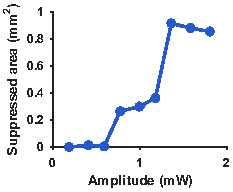
\includegraphics[width=0.34\linewidth]{images/supplementary/imp_spatial_area.pdf}
    \caption{\textbf{Spatial spread of optogenetic inhibition with laser power}
    (AL\_0033, 2025-01-29). Suppressed area against stimulation amplitude, where
    a pixel counts as suppressed if its background-corrected response falls below
    half the median response within $0.2$\,mm of the peak at the strongest
    amplitude; background is the mean over an annulus $0.6$--$0.9$\,mm from that
    peak. The relationship is a threshold rather than a gradual widening: the
    area is negligible below $0.6$\,mW, rises in two steps, and plateaus near
    $0.9$\,mm$^2$ above $1.4$\,mW. Because the threshold is referred to the
    strongest amplitude, these areas are relative and should not be read as an
    absolute extent of opsin activation. Per-amplitude maps are in
    Fig.~\ref{fig:spatial_maps}.}
    \label{fig:spatial_spread}
\end{figure}

\begin{figure}[h]
    \centering
    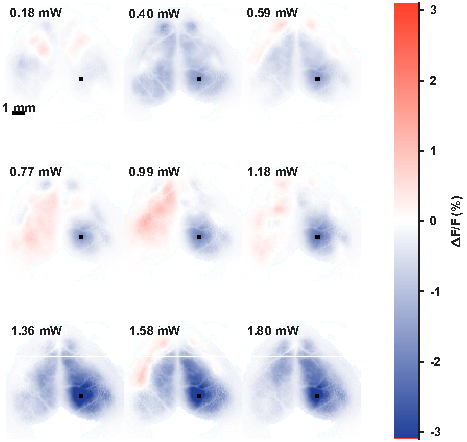
\includegraphics[width=0.72\linewidth]{images/supplementary/imp_spatial_maps.pdf}
    \caption{\textbf{Mean response maps across stimulation amplitudes}
    (AL\_0033, 2025-01-29). Trial-averaged $\Delta F/F$ (\%) over 0--200\,ms
    post-onset at each of the nine delivered amplitudes, masked to the brain and
    drawn on a symmetric blue--white--red scale so that zero is white and
    suppression is blue. Black square, the $10\times10$\,pixel readout kernel at
    the stimulation site. Scale bar, $1$\,mm (pixel scale $0.0173$\,mm). A focal
    suppression at the stimulation site deepens with laser power. Two features of
    these maps are not focal: a positive deflection appears over the opposite
    hemisphere at intermediate powers, and at the highest powers the suppression
    extends bilaterally, so the response at a given pixel is not a pure readout
    of local opsin activation
    %% FILL: citation for graded spatial recruitment of Chrimson. The old draft
    %% carried a red \todo here that was visible in the compiled PDF.
    .}
    \label{fig:spatial_maps}
\end{figure}

\begin{figure}[!ht]
    \centering
    \begin{subfigure}[t]{0.49\linewidth}
        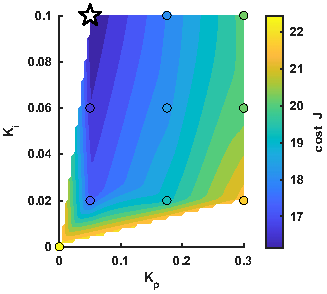
\includegraphics[width=\linewidth]{images/tuning/grid_cost_surface_AL_0033_0305.pdf}
        \caption*{\textbf{A}}
    \end{subfigure}
    \hfill
    \begin{subfigure}[t]{0.49\linewidth}
        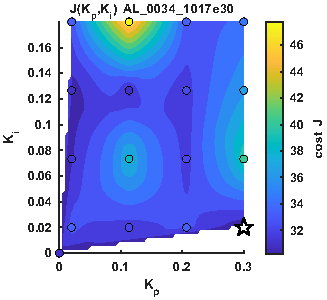
\includegraphics[width=\linewidth]{images/tuning/grid_cost_surface_AL_0034_1017.pdf}
        \caption*{\textbf{B}}
    \end{subfigure}
    \\[0.5em]
    \begin{subfigure}[t]{\linewidth}
        \centering
        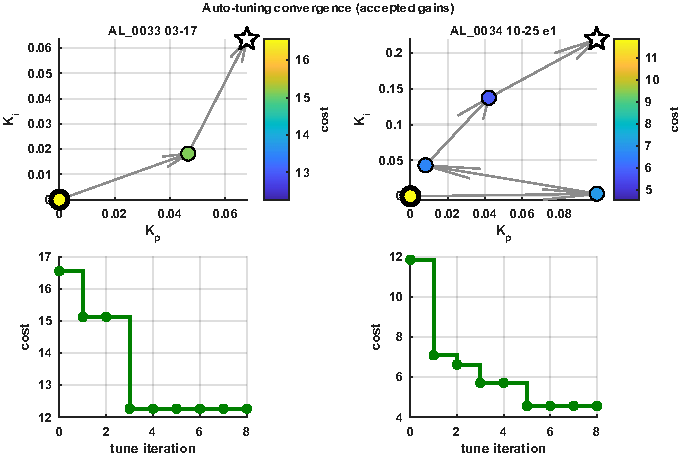
\includegraphics[width=0.92\linewidth]{images/tuning/autotune_convergence_both.pdf}
        \caption*{\textbf{C}}
    \end{subfigure}
    \caption{\textbf{Controller gain tuning.}
        \textbf{A:} Empirical cost surface $\hat{J}(K)$ over a grid of fixed PI
        gains in a representative session (AL\_0033, 2025-03-05), with a single
        low-cost basin and its minimum marked.
        \textbf{B:} An independent grid in a second mouse (AL\_0034, scored over
        its 4\,s stimulation window) recovers the same low-cost region.
        \textbf{C:} Online zeroth-order tuning in both mice: the accepted gain
        trajectory $(K_p, K_i)$ and the running cost against iteration. Cost
        descends in each mouse, and in AL\_0033 the auto-tuned gains settle
        inside the basin identified by the grid in A.}
    \label{fig:cost_landscape}
\end{figure}

\begin{figure}
    \centering
    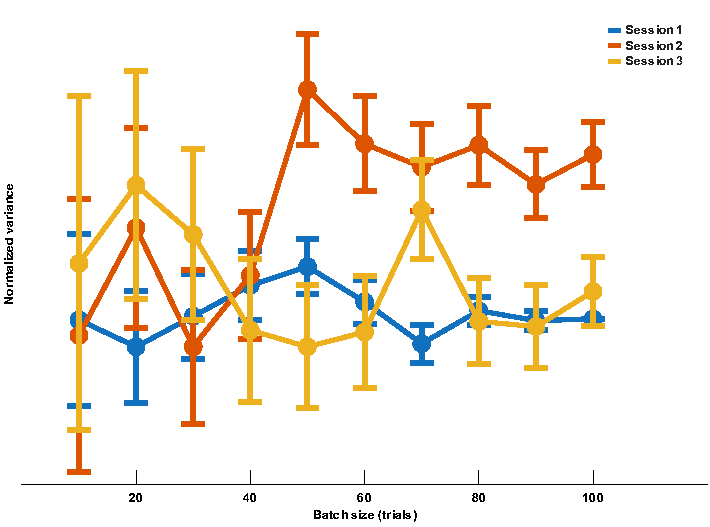
\includegraphics[width=0.46\linewidth]{images/supplementary/spont_variance.pdf}
    \caption{\textbf{Cross-trial variance converges with trial count.} Mean total
    variance $\mathrm{Var}(y_t)$ of spontaneous $\Delta F/F$, averaged across the
    spontaneous window and over five random subsamples per batch size, against
    the number of trials $N$ in the average. Each line is one session. Variance
    stabilizes beyond roughly 50 trials, so the validation blocks are long enough
    to estimate the trial-averaged response.}
    \label{fig:S1}
\end{figure}

\begin{figure}
    \centering
    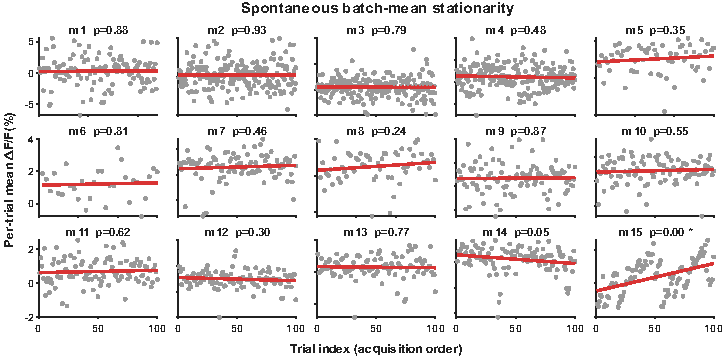
\includegraphics[width=\linewidth]{images/supplementary/batch_mean_stationarity.pdf}
    \caption{\textbf{The spontaneous mean is stationary across acquisition
    order.} Per-trial mean spontaneous $\Delta F/F$ (gray) against trial index
    for each session, with an ordinary least-squares fit (red) and its $p$-value.
    Variance convergence alone would also follow from a slowly drifting mean; the
    absence of a trend rules that out and supports the zero-mean disturbance
    assumption behind Assumption~\ref{assm:trial_avg}.}
    \label{fig:S2}
\end{figure}

\begin{figure}
    \centering
    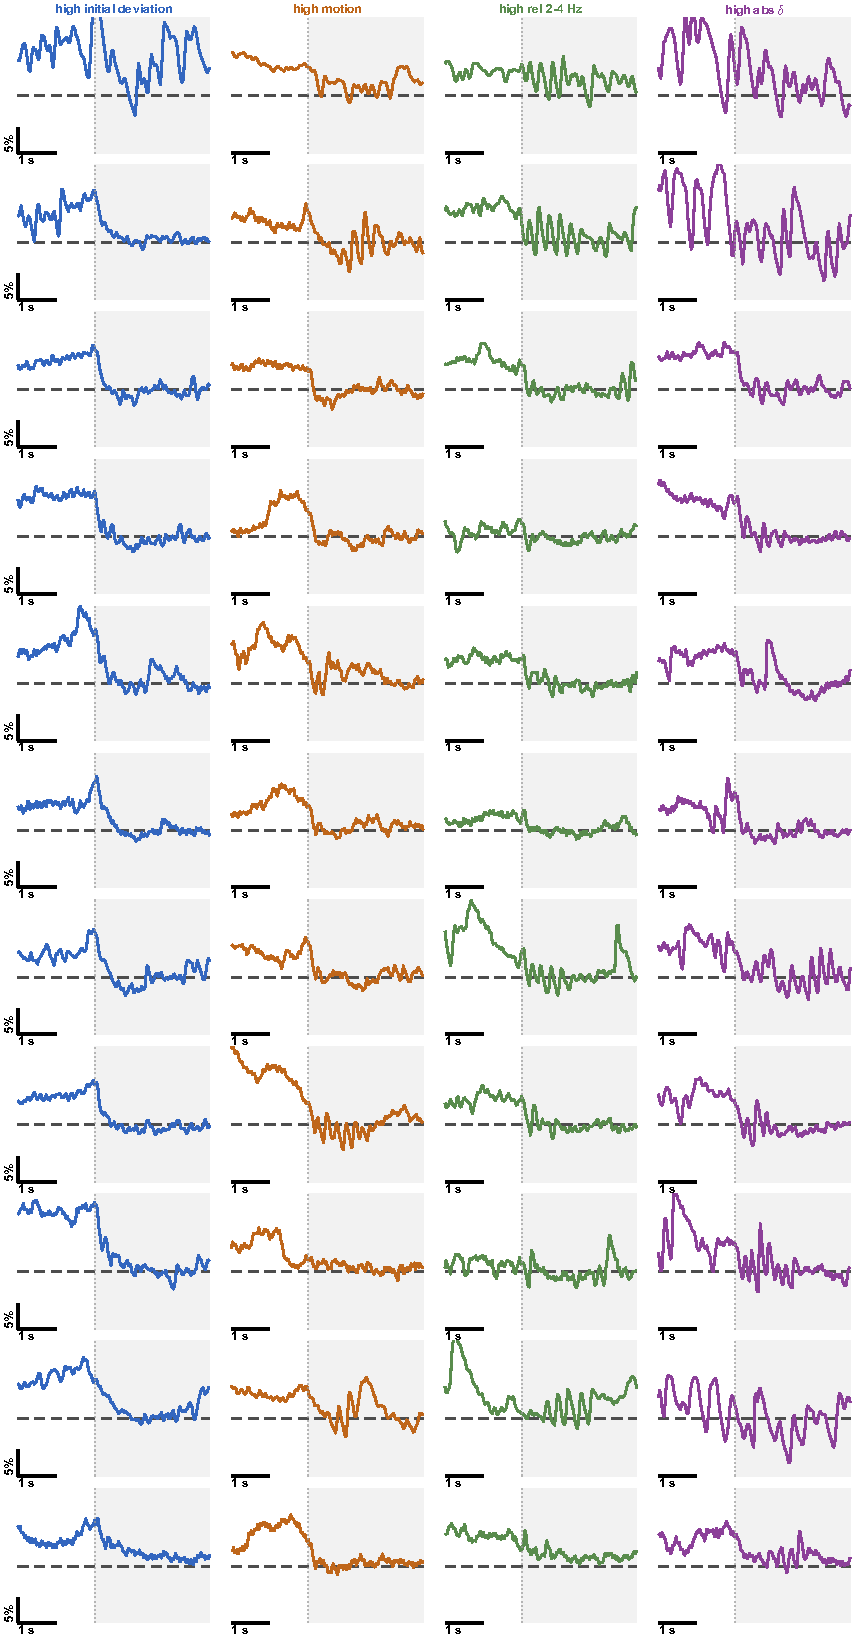
\includegraphics[width=0.9\linewidth]{images/supplementary/f4_exemplars_sessions.pdf}
    \caption{\textbf{State exemplars are consistent across sessions.} For every
    session with motion capture (rows), a representative closed-loop trial for
    each of four pre-stimulus states (columns: high initial deviation, high
    motion, high relative 2--4\,Hz power, high absolute 2--4\,Hz power), chosen as
    the trial highest in that state and low in the others within that session.
    Colors match Fig.~\ref{fig:figure4}A. Dashed line, reference
    ($-5\%\,\Delta F/F$); shading, stimulation window; scale bars 1\,s and 5\%.
    The main-text exemplars in Fig.~\ref{fig:figure4}A are representative of the
    same patterns.}
    \label{fig:S3}
\end{figure}

\begin{figure}
    \centering
    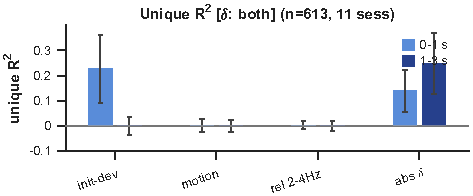
\includegraphics[width=0.32\linewidth]{images/supplementary/f4_decomp_unique_both.pdf}\hfill
    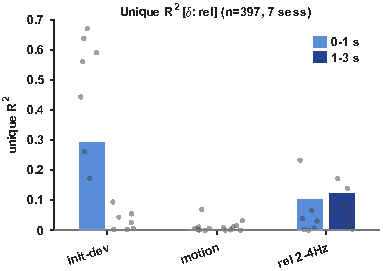
\includegraphics[width=0.32\linewidth]{images/supplementary/f4_decomp_unique_rel.pdf}\hfill
    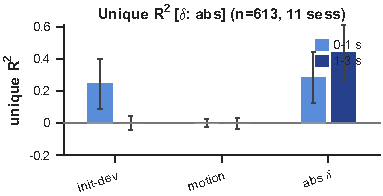
\includegraphics[width=0.32\linewidth]{images/supplementary/f4_decomp_unique_abs.pdf}
    \caption{\textbf{The error decomposition does not depend on how the
    low-frequency factor is defined.} Unique $R^2$ of each state factor for
    closed-loop tracking error, in the transient (0--1\,s) and steady-state
    (1--3\,s) windows, under three specifications of the low-frequency term: relative and
    absolute 2--4\,Hz power entered together (left), relative only (middle), and
    absolute only (right). The main text (Fig.~\ref{fig:figure4}C) enters each
    low-frequency term in its own initial-deviation-plus-motion base, which
    avoids the collinearity that suppresses the relative term when both are
    forced into one model (left). In every specification the initial deviation
    owns the transient window, the low-frequency term carries the steady-state window,
    and motion contributes little.}
    \label{fig:S4}
\end{figure}

% =============================================================================
% REMOVED: contralateral ARX model.
%
% Nothing in results.tex or discussion.tex cites this subsection. It described the
% analysis behind the parked Figure 4 panel A. Restore it if that panel comes
% back; delete it if the panel is retired.
%
% \subsubsection*{Contralateral ARX model}
%
% To quantify how much of the ipsilateral readout is explained by contralateral
% dynamics and by the optogenetic input, we fitted a linear autoregressive model
% with exogenous inputs to wide-field data from spontaneous blocks. The model
% regressed the ipsilateral readout on lagged contralateral pixels selected by a
% spatial cross-correlation criterion. We evaluated fit by $R^2$ on a held-out
% 20\% test set and required $R^2 > 0.3$ on spontaneous data for a session to
% enter the prediction layers. We compared three nested layers: contralateral
% pixels alone; contralateral pixels plus the session-averaged open-loop impulse
% response; and contralateral pixels plus the per-trial laser command convolved
% with the fitted transfer function.
% =============================================================================
